\chapter{Exploratory Development and Experimental Methodology}
\label{chap:methodology}

\section{Two phases of evidence}

The project contains two qualitatively different forms of evidence. During the
\emph{exploratory phase}, individual runs were used to expose implementation
problems, compare broad architectural directions, and generate new hypotheses.
This phase produced the evolution of the FAM, the SSJ regularizer, extensions
to Deformable DETR, and a complete DINO implementation. Its numerical results
describe the development history but do not estimate run-to-run variability
under a common final protocol.

The subsequent \emph{locked-protocol phase} was motivated by the observation
that repeated executions could change the ranking of configurations. In this
phase, the main RT-DETR hypotheses were evaluated with five paired seeds,
fixed training duration, final checkpoints, isolated processes, consistent
initialization, and aggregate reporting. The distinction is retained throughout
the thesis: exploratory evidence motivates a test, whereas locked-protocol
evidence supports the principal comparison.

\begin{figure}[H]
  \centering
  \thesisimage[\textwidth]{images/experimental_timeline.pdf}{Timeline from the inherited course-project baseline, through post-coursework exploration and the variability audit, to the final RT-DETR and YOLOv10 protocols.}
  \caption{Chronology and evidential status of the study. The first two stages
  establish the inherited starting point and record hypothesis-generating work
  conducted under the previous protocol. The audit motivates the redesign, while the
  horizontal separator marks the transition to the locked RT-DETR and YOLOv10
  multi-seed evaluations.}
  \label{fig:experimental-timeline}
\end{figure}

\section{Post-coursework evolution of the FAM}
\label{sec:fam-history}

\subsection{Lazy registration bug}

The first RT-DETR FAM implementation instantiated its alignment layers lazily
during the first forward pass. The optimizer was created earlier and therefore
did not contain those parameters. The offset predictor remained at zero, while
the deformable-convolution weights remained fixed at their random
initialization. This model did not implement an identity transformation and did
not train a functional FAM, even though its fusion score was high in one run.

The extremely low IR-only score of that checkpoint is consistent with a weak
or unusable thermal path, but the final metrics do not prove literal
cancellation of the IR backbone. The run is useful as a debugging case, not as
a competitive model.

\subsection{Eager, Frozen, and Spatial Dropout variants}

The implementation was corrected by registering all FAM layers in the model
constructor before optimizer creation. This \emph{Eager FAM} allowed the
alignment parameters to train from the first optimization step. A Frozen
variant then tested a fixed, eagerly registered transform: gradients could
propagate through it to the IR backbone, but the FAM parameters themselves did
not change. A further variant applied channel-wise spatial dropout to the
transformed IR features immediately before addition.

These interventions did not isolate a single causal explanation for the
historical Lazy score. In particular, the Lazy bug generated a fixed random
filter with null offsets, not stochastic geometric jitter. Their role was to
motivate a cleaner hypothesis about perturbing sampling geometry during
training.

\subsection{Stochastic Spatial Jitter}

Stochastic Spatial Jitter adds zero-mean Gaussian noise to the predicted
offsets only during training:

\begin{equation}
  \Delta_{\mathrm{train}}=\Delta_{\mathrm{FAM}}+\varepsilon,
  \qquad \varepsilon\sim\mathcal{N}(0,\sigma^2).
  \label{eq:ssj}
\end{equation}

Unlike feature dropout, SSJ does not explicitly remove channels. It perturbs
the positions sampled by DCNv2 around the correction currently predicted by
the FAM. At inference, \(\varepsilon\) is absent. The intended regularization
is therefore local uncertainty around a learned transformation, rather than a
return to the original sensor displacement.

\Cref{tab:fam-historical} reports the single-run results that generated the
SSJ hypothesis. They are deliberately separated from the final comparison.

\begin{table}[H]
  \centering
  \caption{Historical single-run FAM development results. These values represent the \mapfifty{}
  scores of the exploratory phase and do not determine the final model selection.}
  \label{tab:fam-historical}
  \begin{adjustbox}{max width=\textwidth}
  \begin{tabular}{lccc}
    \toprule
    Variant & VIS & IR & VIS+IR \\
    \midrule
    Lazy registration bug & 0.3000 & 0.0054 & 0.4286 \\
    Eager FAM & 0.2620 & 0.2629 & 0.3960 \\
    Frozen FAM & 0.2517 & 0.2250 & 0.3857 \\
    Eager FAM + 40\% Spatial Dropout & 0.2716 & 0.2248 & 0.3936 \\
    Eager FAM + SSJ & 0.2697 & 0.1818 & 0.4381 \\
    \bottomrule
  \end{tabular}
  \end{adjustbox}
\end{table}

The SSJ run reached the largest historical fusion value, but its apparent
advantage did not survive paired replication: the locked-protocol result in
\Cref{sec:rtdetr-main-results} selects the standard FAM without SSJ.

\section{Exploratory architectural extensions}

\subsection{Deformable DETR with channel fusion, FAM, and SSJ}
\label{sec:defdetr-exploration}

The inherited Deformable DETR adaptation uses independent ResNet-50 RGB and IR
backbones. The IR input stem is initialized by averaging the three RGB input
channels. At the three native backbone levels, corresponding features are
concatenated along the channel dimension and passed through a nonlinear fusion
block:

\begin{equation}
  F^{(i)}_{\mathrm{fused}}=
  \operatorname{ReLU}\!\left(
  \operatorname{GN}_{32}\!\left(
  \operatorname{Conv}_{1\times1}
  ([F^{(i)}_{\mathrm{RGB}},F^{(i)}_{\mathrm{IR}}])
  \right)\right).
  \label{eq:defdetr-channel-fusion}
\end{equation}

The model retains the standard four-scale Deformable DETR configuration. The
three native ResNet levels (C3,C4,C5) are fused explicitly; a fourth level is
then derived from the fused (C5) feature through a stride-2 projection. This
is the usual multi-scale construction of Deformable DETR, rather than an
additional backbone output. The pretrained configuration retains six
deformable-attention encoder layers and six decoder layers.

This preserves the spatial dimensions required by the pretrained attention
reference points. It replaced an unsuccessful spatial-concatenation attempt
that doubled feature-map height, forced a reduction in pyramid levels because
of memory use, and produced near-zero detection performance.

In a previous project we had already integrated FAM before the channel
fusion block, while here we extend it by adding SSJ under the same previous
experimental regime. Five runs are available for each configuration, but they
precede the final RT-DETR head initialization, checkpoint rule, and validation
policy. Their median and range are reported in
\Cref{tab:defdetr-exploratory} as exploratory transfer evidence.

The architecture is divided across
\Cref{fig:defdetr-fusion-frontend,fig:defdetr-backend} to keep both the
multimodal processing and the standard detector components legible. The first
diagram follows the RGB--IR streams through the optional FAM, channel fusion,
four-level projection, and multi-scale flattening. The second continues from
that token sequence through the standard single-stage Deformable DETR encoder,
learned queries, decoder, and prediction heads. SSJ is not shown because it is
used only during training and does not modify the inference graph.

\begin{figure}[H]
  \centering
  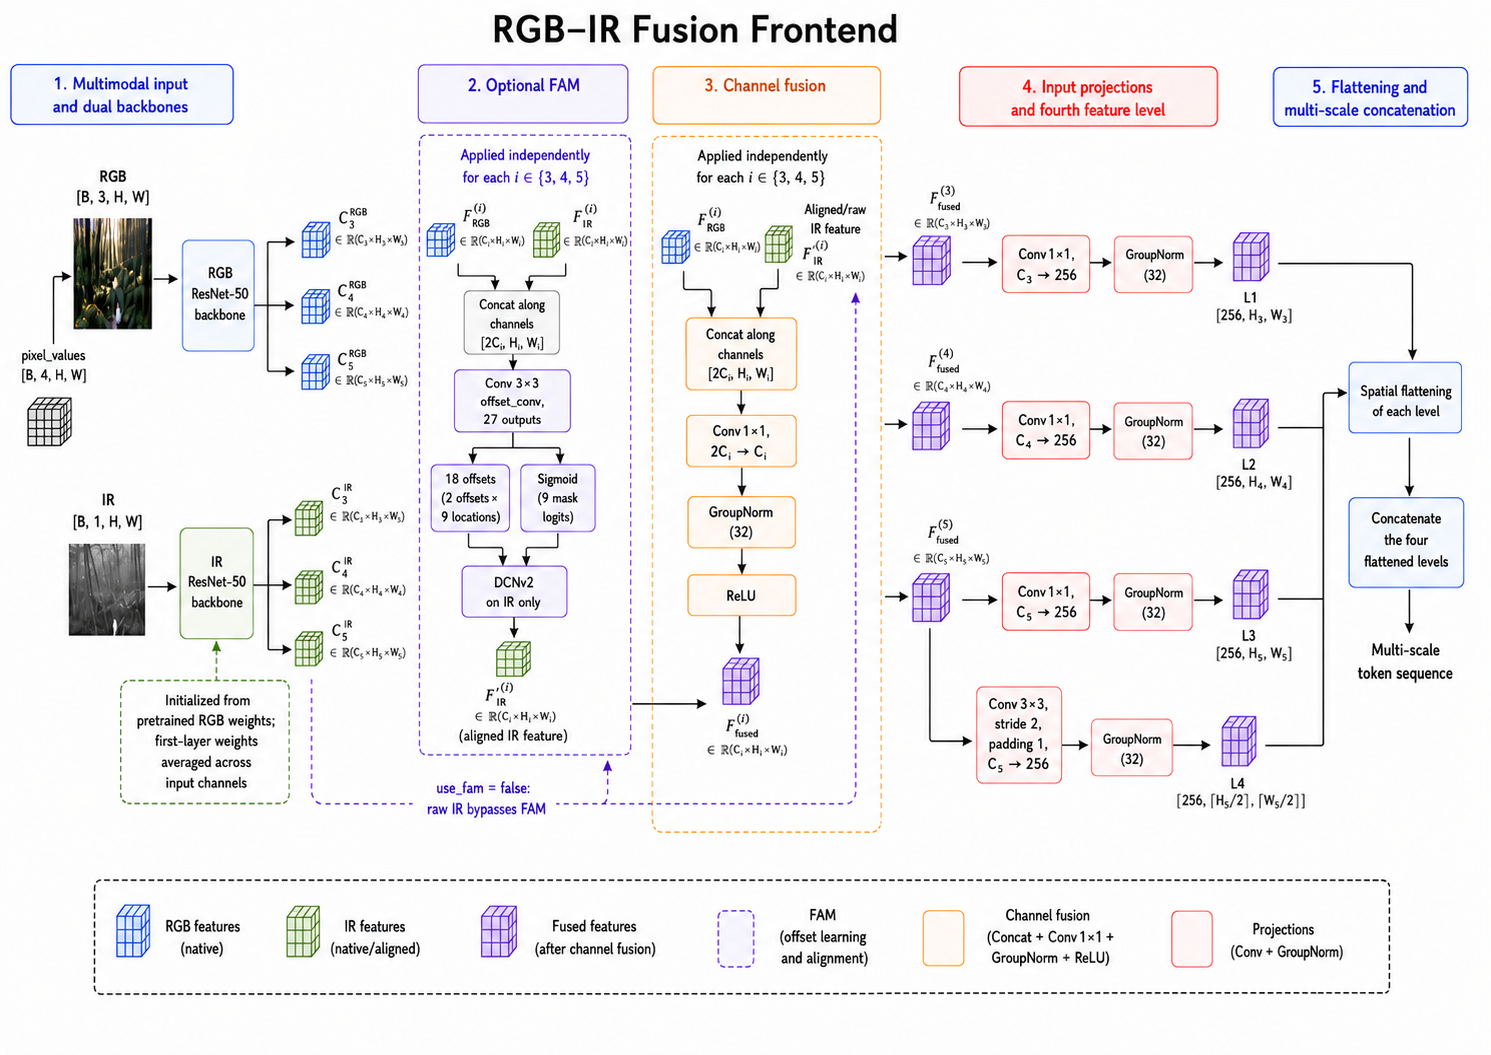
\includegraphics[width=\textwidth]{images/frontend_defdetr.png}
  \caption{RGB--IR frontend of the dual-backbone Deformable DETR adaptation.
  FAM is applied independently to the three native feature levels when
  enabled, otherwise the raw IR features bypass it. Each RGB--IR pair is then
  fused along the channel dimension. The fourth encoder level is generated
  from the fused C5 feature and therefore does not receive a separate FAM.}
  \label{fig:defdetr-fusion-frontend}
\end{figure}

\begin{figure}[H]
  \centering
  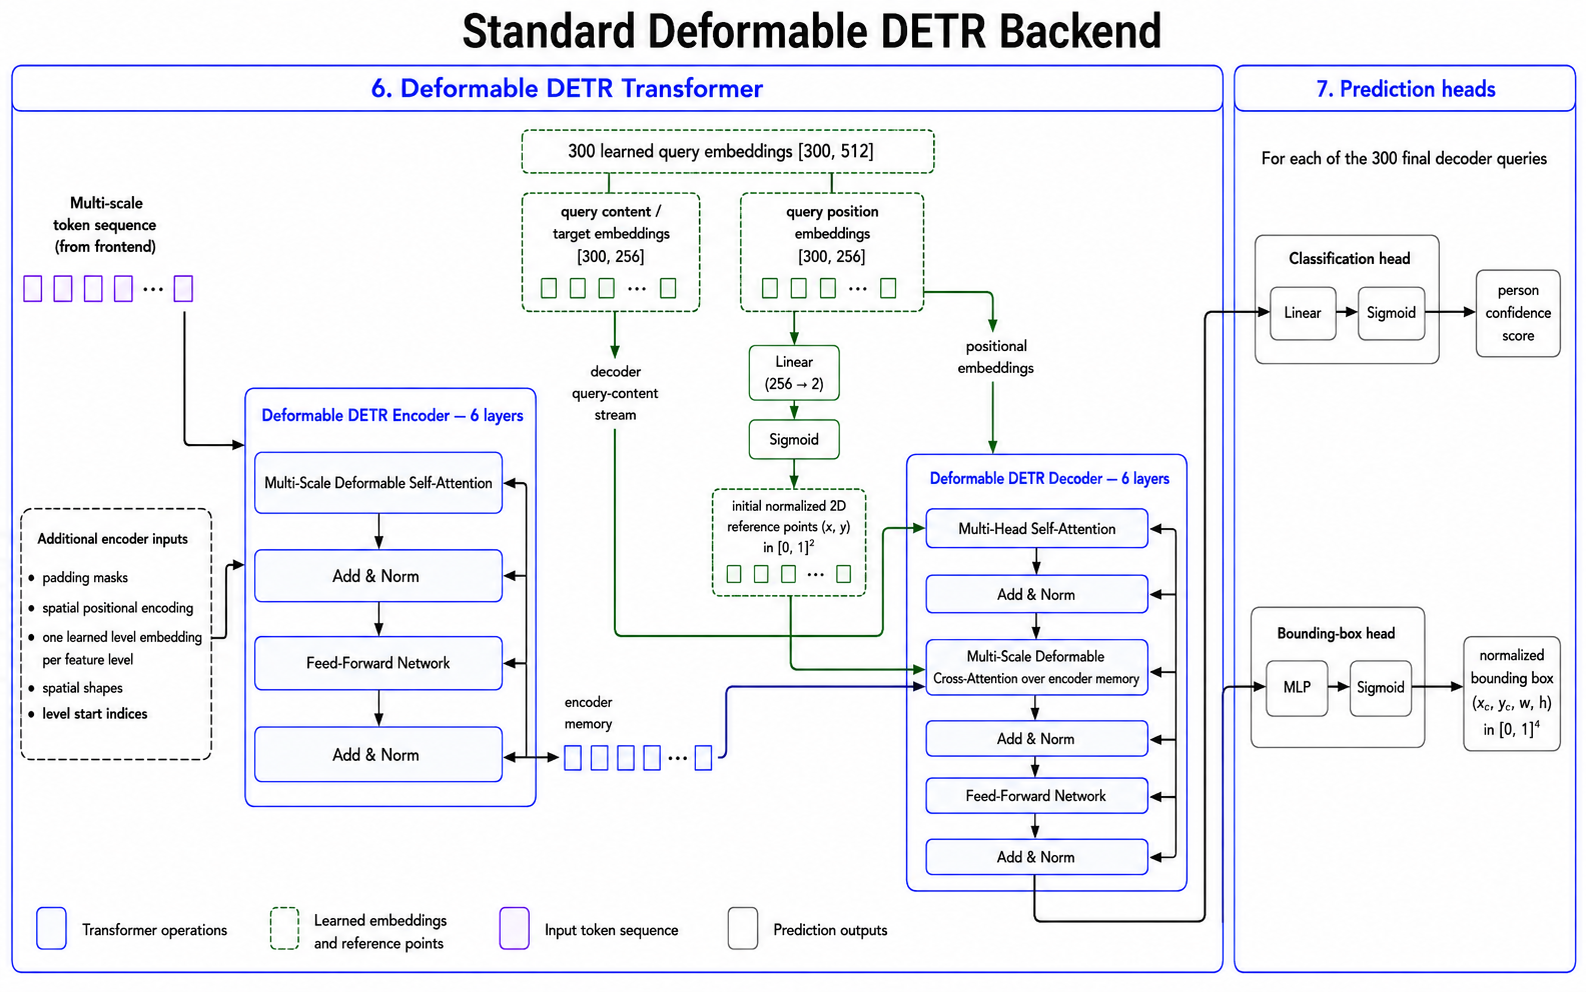
\includegraphics[width=\textwidth]{images/backend_defdetr.png}
  \caption{Standard single-stage Deformable DETR backend used after the
  multimodal frontend. The four flattened feature levels enter the
  deformable-attention encoder. Learned query content, positional embeddings,
  and reference points then condition the decoder, whose final outputs feed
  the classification and bounding-box heads.}
  \label{fig:defdetr-backend}
\end{figure}

\begin{table}[H]
  \centering
  \caption{Exploratory Deformable DETR results, reported as median
  [minimum--maximum] \mapfifty{} over five runs.}
  \label{tab:defdetr-exploratory}
  \begin{tabular}{lccc}
    \toprule
    Configuration & VIS & IR & VIS+IR \\
    \midrule
    Deformable DETR & 0.157 [0.131--0.197] & 0.115 [0.086--0.142] & 0.249 [0.199--0.303] \\
    + FAM & 0.184 [0.171--0.253] & 0.131 [0.097--0.165] & 0.294 [0.213--0.314] \\
    + FAM + SSJ & 0.142 [0.115--0.206] & 0.088 [0.073--0.109] & 0.263 [0.170--0.350] \\
    \bottomrule
  \end{tabular}
\end{table}

FAM has the highest observed median, but the ranges overlap substantially.
SSJ does not reproduce the gain suggested by the preliminary RT-DETR run and
has the widest VIS+IR range. A definitive cross-architecture ranking would
require retraining these models under a protocol aligned with the final
RT-DETR study.

\subsection{Complete DINO implementation}
\label{sec:dino-exploration}

The complete DINO implementation retains the dual-backbone and channel-fusion
base of Deformable DETR: four feature levels, six encoder layers, and six
decoder layers. It activates all three defining mechanisms. MQS uses the top
encoder proposals as spatial anchors while drawing query content from an
independent learned embedding. LFT keeps the refined reference passed to the
next attention layer detached while preserving a graph-connected copy for the
following prediction loss. CDN inserts noisy positive and negative target
queries during training and applies the required decoder attention mask.

The complete implementation was trained five times and produced the values in
\Cref{tab:dino-exploratory}. Since even its maximum fusion result remained
below the median of the historical Deformable DETR base, complete FAM and SSJ
variants were not launched without a new diagnostic hypothesis.

\begin{table}[H]
  \centering
  \caption{DINO base result under the previous protocol, reported as
  median [minimum--maximum] \mapfifty{} over five runs.}
  \label{tab:dino-exploratory}
  \begin{tabularx}{\textwidth}{@{}l *{3}{>{\centering\arraybackslash}X}@{}}
    \toprule
    Configuration & VIS & IR & VIS+IR \\
    \midrule
    Complete DINO base
      & \shortstack{0.0565\\{\footnotesize [0.0232--0.1091]}}
      & \shortstack{0.0881\\{\footnotesize [0.0671--0.1473]}}
      & \shortstack{0.1088\\{\footnotesize [0.0669--0.1635]}} \\
    \bottomrule
  \end{tabularx}
\end{table}

This is a negative result for the implemented configuration and training
budget, while it does not show that DINO is intrinsically unsuitable for WiSARD.

\section{Reproducibility investigation}
\label{sec:reproducibility}

\subsection{Why single runs were insufficient}

Two native-CUDA RT-DETR training runs with the same nominal seed and pretrained
person head produced final test \mapfifty{} values of 0.4171 and 0.2934. Their
first forward loss was identical, but their weight hashes diverged after the
first backward pass. A difference of 0.1236 is large enough to reverse many of
the historical architectural comparisons.

The investigation therefore recorded runtime fingerprints, initialization
hashes, sample indices, modality-dropout decisions, input hashes, losses, and
post-update weight hashes. Native execution diverged at the first optimizer
step even when inputs and the initial loss matched. A deterministic
interpolation substitute for the deformable-attention sampling path produced
identical traces, metrics, and final checkpoint hashes in two complete
RT-DETR runs. This establishes that strict reproduction is possible for that
substitute path, while native RT-DETR CUDA is not fully deterministic.

\subsection{Pretrained single-class head}

The original COCO checkpoint has 80 classes, whereas the task has one class,
\emph{person}. Randomly initialized classification and denoising heads made the
seed affect a substantial part of the initial model. The final setup transfers
the COCO person row into all compatible RT-DETR classification heads and the
denoising embedding. This makes the initial model hash independent of the
experiment seed and reduces, but does not eliminate, amplification of native
CUDA perturbations.

In 20-step probes, the mean range of the loss across identical-seed native
runs decreased from 4.0763 with random heads to 0.4393 with the transferred
person head. The maximum range decreased from 20.8075 to 1.6424. The change is
therefore a mitigation and a more controlled transfer-learning initialization,
not a determinism guarantee.

\subsection{DCNv2 deterministic limitation}

The strict FAM probe stops at the first backward pass because the CUDA backward
of \texttt{torchvision.ops.DeformConv2d} has no deterministic implementation in
the studied environment. A numerically equivalent PyTorch fallback was too
slow at the 512, 1024, and 2048 channel feature levels for full training. FAM
must consequently be evaluated statistically under native CUDA rather than
through a strictly deterministic full campaign.

\subsection{Modal Dropout and evaluation leakage}

The data pipeline originally sampled Modal Dropout during validation and test
as well as training. This made evaluation inputs stochastic and inconsistent
with the intended VIS, IR, and VIS+IR conditions. The loader was corrected and
regression-tested so that dropout is active only in training while all final
evaluations disable it.

\subsection{Validation and checkpoint policy}

The effective validation split contains 273 FHL frames, of which 184 are
empty, and only 148 boxes. Its objects are substantially smaller than those in
training and MtErie. Near-zero validation metrics are therefore evidence of a
domain and scale mismatch, not proof that the validator is defective or that
the split has no information.

Using that split for early stopping does not provide a representative rule for
MtErie. Conversely, choosing an epoch from MtErie would tune directly on the
internal test. The final RT-DETR protocol resolves the immediate comparison by
fixing ten epochs in advance and evaluating the final \texttt{latest}
checkpoint. Validation is not run as a selector and this does not replace the need
for a future representative train-derived validation set.

\section{Locked RT-DETR protocol}
\label{sec:locked-rtdetr-protocol}

The final RT-DETR comparison uses six independently trained configurations:

\begin{enumerate}[label=\arabic*.]
  \item Base (direct additive fusion);
  \item standard FAM with DCNv2;
  \item FAM with IR feature dropout probability 0.4;
  \item FAM with SSJ standard deviation 0.5;
  \item an identity-initialized DCNv2 FAM;
  \item a direct bilinear Grid Sample warp.
\end{enumerate}

IR feature dropout is active only during training. Immediately after FAM has
transformed the IR feature map and before additive fusion, \texttt{Dropout2d}
independently zeros complete IR feature channels with probability 0.4 at each
pyramid level; the remaining channels are rescaled in the usual way. It does
not remove complete frames or disable the IR sensor, and it is inactive during
all evaluations.

The identity DCNv2 ablation retains the standard FAM structure but initializes
the central kernel as a channel-wise identity with weight two, exactly
compensating the initial mask value 0.5. The Grid Sample variant predicts one
two-dimensional displacement per spatial cell and applies a bilinear warp
without a learned post-sampling convolution. It is exactly the identity at
zero offset through a correction that subtracts numerical sampling of the base
grid.

\begin{table}[H]
  \centering
  \caption{Locked RT-DETR protocol used by all six final configurations.}
  \label{tab:rtdetr-protocol}
  \begin{tabularx}{\textwidth}{lX}
    \toprule
    Component & Fixed choice \\
    \midrule
    Training seeds & Paired seeds 40--44; five runs per configuration \\
    Execution & Native CUDA; one isolated Python process per seed \\
    Training horizon & 10 fixed epochs \\
    Checkpoint & Final \texttt{latest}; no test-based or validation-based selection \\
    Initialization & Pretrained RT-DETR R50vd and transferred COCO person heads \\
    Transformer depth & One AIFI encoder layer and six decoder layers \\
    Modal Dropout & VIS/IR/fusion probabilities 0.2/0.2/0.6, training only \\
    Validation & Not used during training or for checkpoint selection \\
    Primary benchmark & MtErie internal development benchmark \\
    Primary metric & \mapfifty{} \\
    Evaluation & VIS, IR, and VIS+IR with a fixed evaluation seed \\
    \bottomrule
  \end{tabularx}
\end{table}

The same seed index is paired across configurations to reduce the noise in
architectural contrasts, while it does not make native executions deterministic.

\section{Statistical reporting}

For every final configuration, the thesis reports all five seed values, mean,
median, sample standard deviation, minimum--maximum range, and a Student
\(t\)-interval for the mean. Architectural contrasts use within-seed
differences, their mean and interval, and the number of paired wins. Paired
\(t\)-tests and exact Wilcoxon signed-rank tests are included as exploratory
summaries.

With only five pairs, intervals are imprecise, p-values are discrete or
sensitive to assumptions, and no correction is applied for the many possible
comparisons. Conclusions therefore prioritize effect size, sign consistency,
and agreement across metrics over a binary significance threshold.

The experimental unit for architectural comparison is the independently
trained run/checkpoint. Frames, bounding boxes, samples used in a diagnostic,
feature-map cells, and the nine DCNv2 kernel points are nested observations,
not independent replicates. Diagnostics first aggregate within a checkpoint
and only then compare the five checkpoints.
